\section{Design}

\begin{figure*}[t]
  \centering
  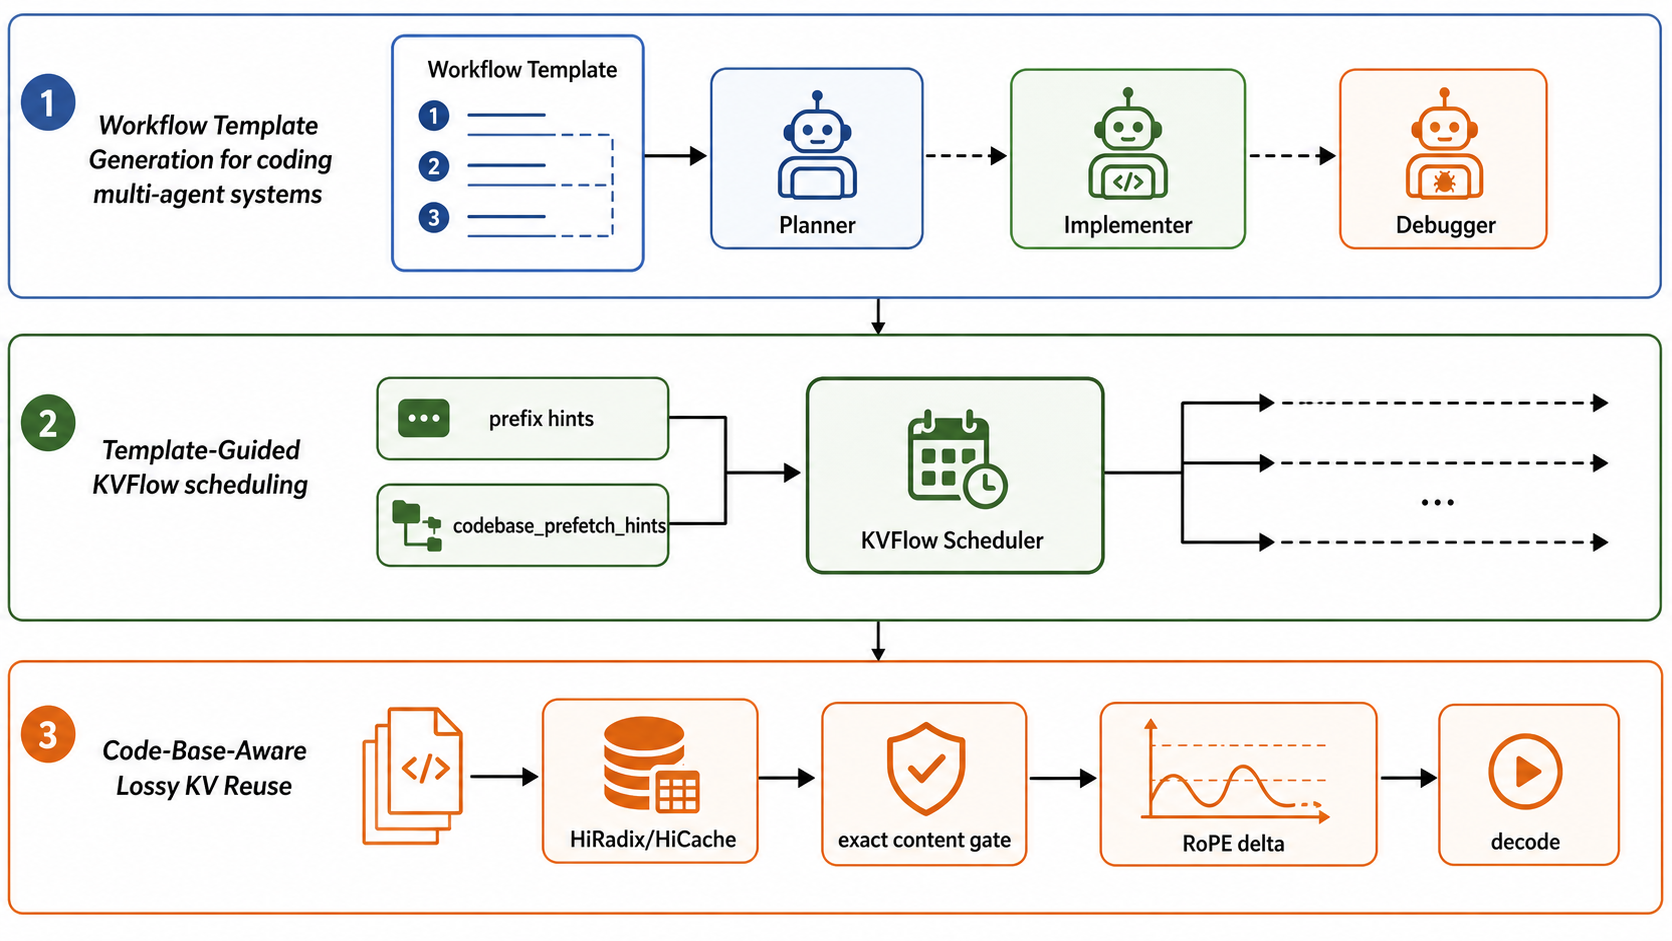
\includegraphics[width=0.94\textwidth]{figures/fig_system_architecture.png}
  \caption{\system overview. Workflow templates expose future agent and code-base accesses; a KVFlow-style scheduler consumes coding-aware prefetch hints; the reuse layer enforces exact-content gates before RoPE-aligned segment reuse.}
  \Description{Three-layer AgentTemplateKV architecture with workflow template generation, KVFlow scheduling, and code-base-aware KV reuse.}
  \label{fig:architecture}
\end{figure*}

\system separates planning, scheduling, and safety.
Figure~\ref{fig:architecture} shows the three-layer architecture.
The template layer describes which agents will run and which code-base segments each agent will need.
The scheduler layer receives this structure as prefetch hints.
The reuse layer decides whether cached KV can be consumed.
The layers communicate through metadata rather than through implicit prompt inspection.
This design is intentional: the MAS controller already knows the workflow roles and the repository files it is about to provide, while the serving engine already owns cache residency, block allocation, and reuse decisions.
\system exposes just enough structure for the engine to prepare useful KV objects, then keeps the final reuse decision inside the engine where tokenization, positions, and cache state are known.

\subsection{Workflow Templates}

A workflow template is a structured description of a coding MAS prompt plan.
For example, a Planner prompt may be:
\[
\{\mathrm{prefix}\} + \{\mathrm{content}_1\} + \{\mathrm{codebase}_1\} + \{\mathrm{codebase}_2\} + \{\mathrm{codebase}_3\}.
\]
An Implementer may later use:
\[
\{\mathrm{prefix}\} + \{\mathrm{context}_2\} + \{\mathrm{codebase}_1\} + \{\mathrm{codebase}_2\}.
\]
A Debugger may use:
\[
\{\mathrm{prefix}\} + \{\mathrm{context}_2\} + \{\mathrm{codebase}_3\} + \{\mathrm{output}\}.
\]
This template makes future exact code-base use visible before every agent request is issued.

Following the original AgentTemplateKV design, templates are produced through multi-round role discovery, tool assignment, DAG construction, and validation.
The current implementation constrains that synthesis for code-base reuse: every reusable object must be a concrete code-base segment with a stable content signature.
The resulting template is not merely a prompt recipe; it is a serving plan containing expected downstream consumers, edge content types, and use distances.
Formally, a template contains an agent DAG $G=(V,E)$ and a set of code objects $C$.
Each object $c \in C$ has a repository identifier, optional path and syntax locator, normalized content signature, estimated token span, producer, and one or more consumer agents.
Edges in $E$ describe how intermediate artifacts such as plans, patches, and test logs move between agents.
Only objects in $C$ are eligible for exact-content segment reuse; other artifacts can still affect prefix-cache locality and scheduling priority, but they do not enter the code-content reuse gate.

This object model lets the same code segment be referenced independently of prompt position.
For example, a Planner and an Implementer may both consume \texttt{file.py:f} even though one prompt places it after the issue description and the other places it after a repair plan.
The template therefore preserves the identity of reusable code across role-specific prompt construction.

\begin{figure}[t]
  \centering
  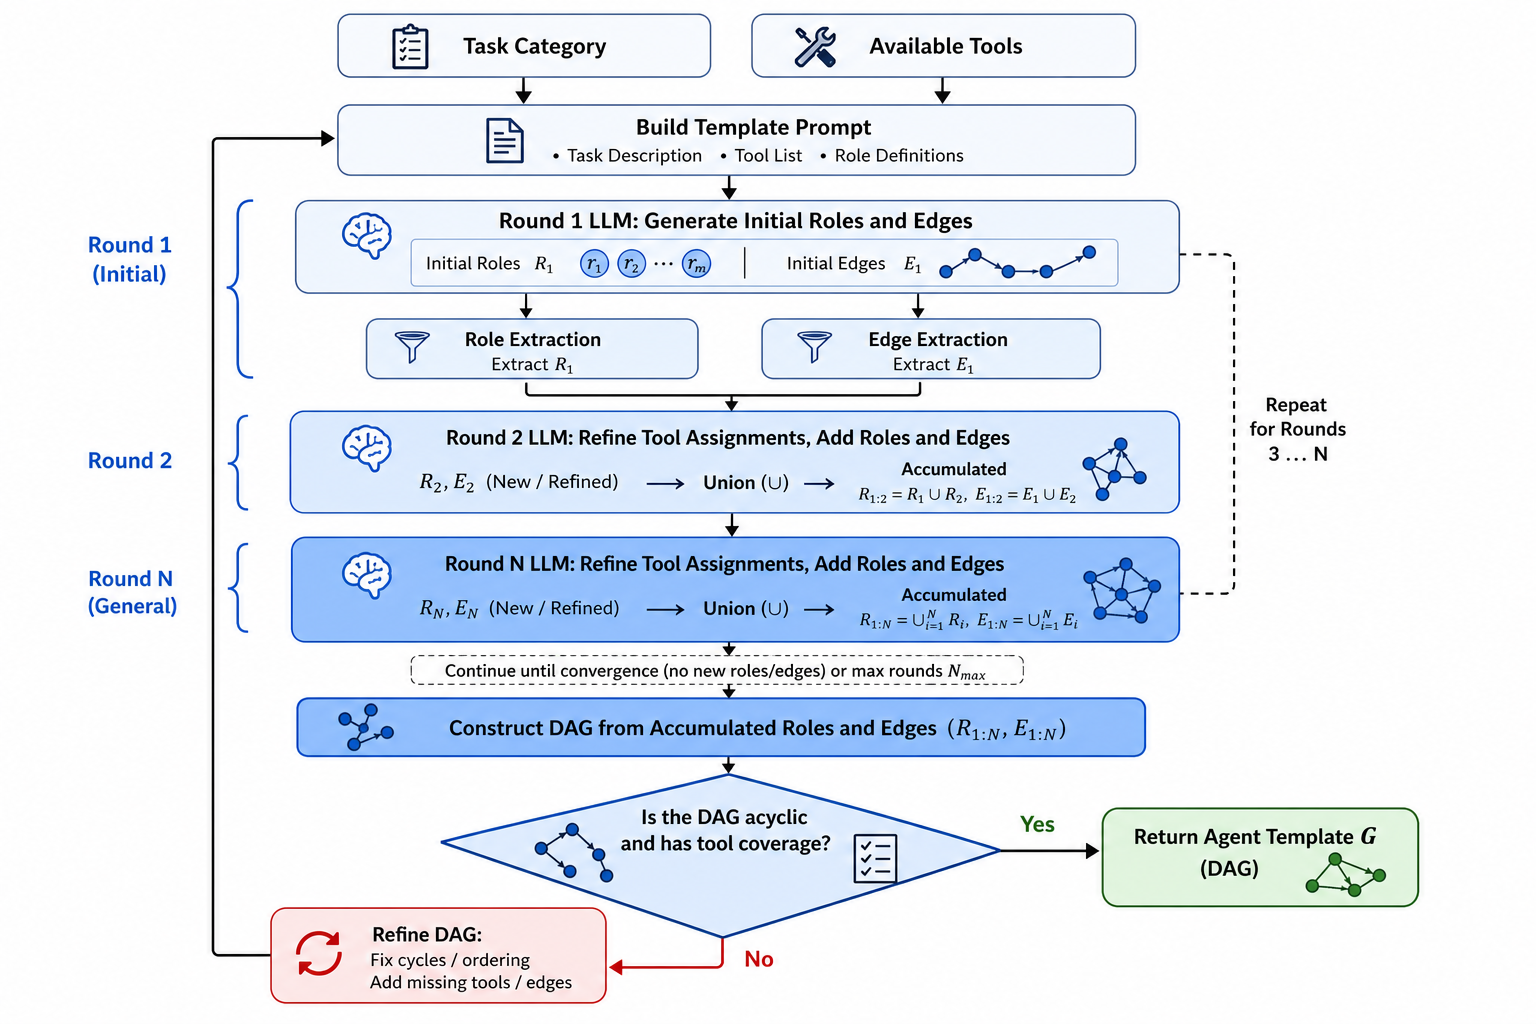
\includegraphics[width=\columnwidth]{figures/fig_template_synthesis_process.png}
  \caption{Template synthesis process inherited from the original project draft and specialized in \system to emit code-base reuse plans.}
  \Description{Template synthesis process with prompt construction, role extraction, DAG validation, and refinement.}
  \label{fig:template-synthesis}
\end{figure}

\subsection{Coding-Aware Scheduling Hints}

The template layer emits \prefetchhint entries with a code-base id, content signature, target agent, use distance, priority, and optional text.
If text is present, the engine may tokenize the exact code block and attempt active prefetch.
If only a signature is present, the engine records the hint for observability and future eviction policy.
In both cases, the hint is not a reuse authorization.
It is a scheduling signal.
The priority field combines workflow distance with content type.
Code segments that will be consumed by the next agent receive higher priority than segments whose next use is several turns away.
Segments consumed by multiple downstream agents are also favored because retaining them can amortize one prefill across several later requests.
These priorities are advisory: under memory pressure the scheduler can evict a hinted segment, and the later request will fall back to normal prefill.

The hint schema also supports partial deployment.
A serving stack that lacks cross-position reuse can still use the metadata for accounting or eviction.
A stack with device-only cache residency can match currently resident code spans but skip host load-back.
A full deployment can combine text-bearing hints, host-backed storage, and exact-content reuse.
The evaluation uses this staged design: it validates the metadata path and exact-content reuse while reporting host-backed prefetch as a limitation.

\begin{figure}[t]
  \centering
  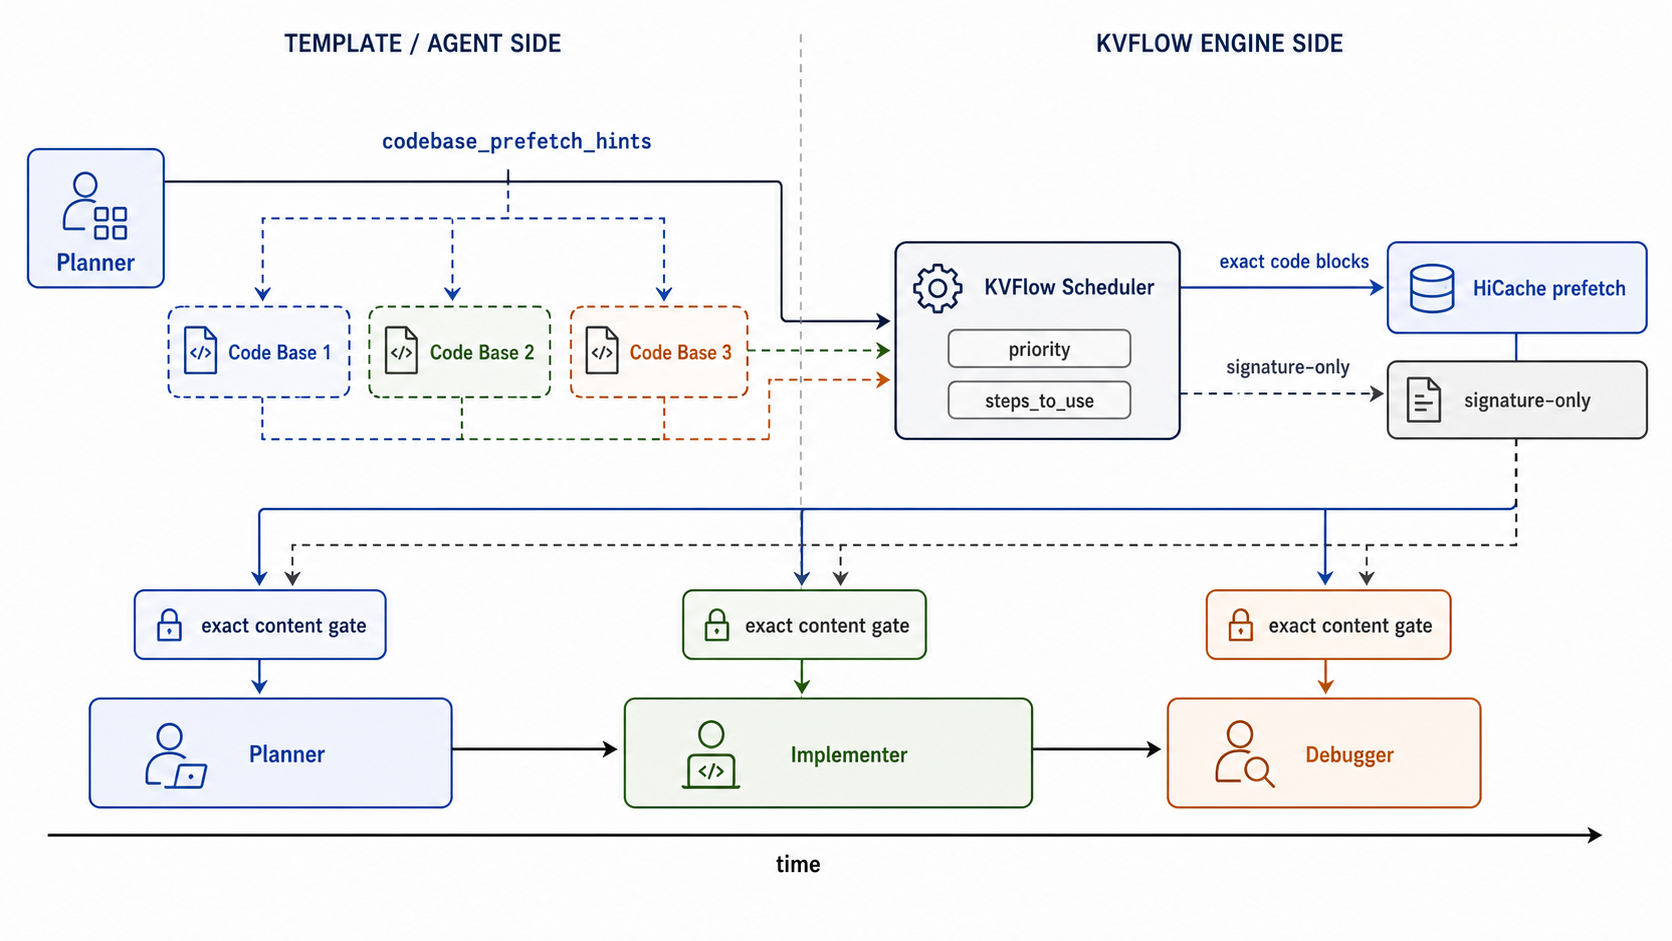
\includegraphics[width=\columnwidth]{figures/fig_coding_prefetch.png}
  \caption{Coding-aware prefetch hints. Templates reveal future code-base use to a KVFlow-style scheduler, while exact-content gates remain responsible for reuse safety.}
  \Description{Timeline showing Planner, Implementer, Debugger, codebase prefetch hints, scheduler, HiCache prefetch, and exact content gate.}
  \label{fig:prefetch}
\end{figure}

\subsection{Exact-Content Segment Reuse}

Figure~\ref{fig:kvcomm} illustrates our code-specific reuse path, which adapts \kvcomm-style cross-context KV reuse to repository code segments.
For each candidate code span, the system records locator metadata and a normalized content signature.
At reuse time, AST and anchors narrow the search, but the final gate compares code content signatures.
Only an exact match permits reuse.
Then the reuse layer applies RoPE delta alignment to the cached K/V tensors before the downstream decode.
The reuse protocol has four steps.
First, the request tokenizer identifies candidate code spans and their target token positions.
Second, locator metadata queries cache entries with compatible repository, path, syntax-region, or anchor signatures.
Third, the exact-content gate compares normalized content signatures and rejects every mismatch.
Fourth, for an accepted match, the engine computes the source-to-target position delta and applies the RoPE transform before exposing the cached tensors to the request.

This protocol deliberately separates two forms of correctness.
Content correctness is discrete: either the normalized code signature matches or the cache entry is unusable.
Positional correctness is numerical: the same code content can be reused at a different position only after alignment.
The evaluation therefore tests both parts separately, using gate ablations for content safety and RoPE/logit ablations for numerical behavior.
Figure~\ref{fig:graph-bundle-method} shows how the graph-aware extension changes candidate selection: the target span is expanded to a bounded one-hop code neighborhood before lookup, while the final exact-content gate is unchanged.

\begin{figure*}[t]
  \centering
  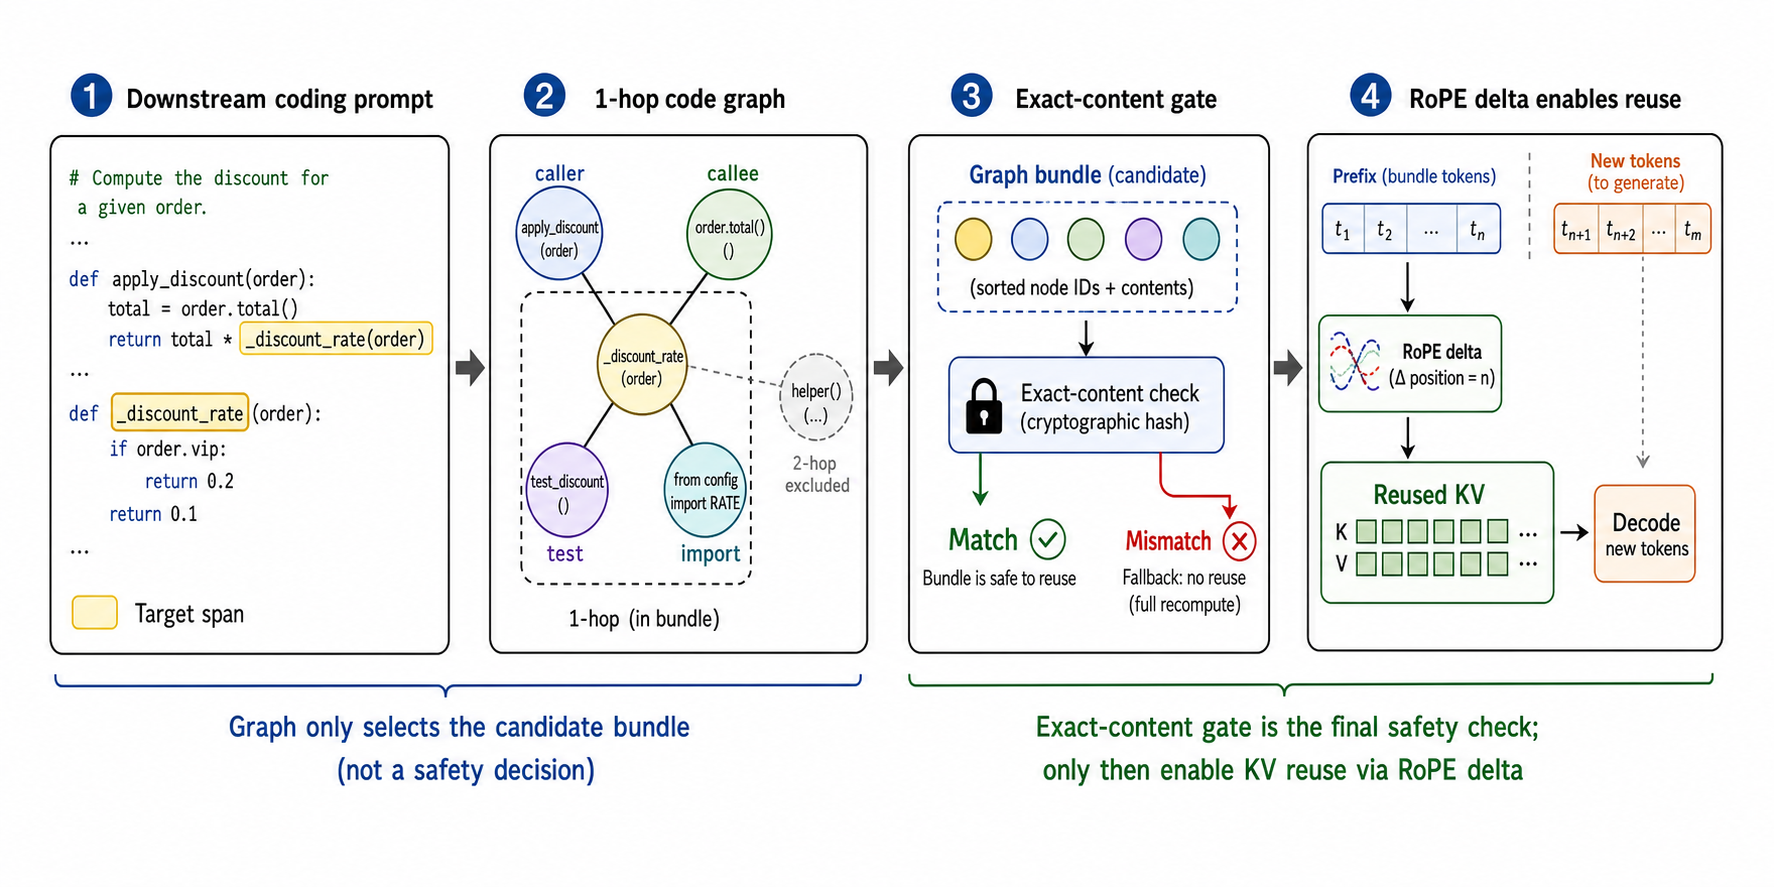
\includegraphics[width=0.98\textwidth]{figures/fig_graph_bundle_method.png}
  \caption{Graph-aware bundle selection. The code graph expands a target span to a one-hop call neighborhood before candidate lookup, but the exact-content signature remains the final reuse gate.}
  \Description{A target code span is expanded to caller, callee, test, and import neighbors in a one-hop graph bundle; a two-hop node is excluded; the bundle then passes through an exact-content gate and RoPE delta alignment before KV reuse.}
  \label{fig:graph-bundle-method}
\end{figure*}

\begin{figure}[t]
  \centering
  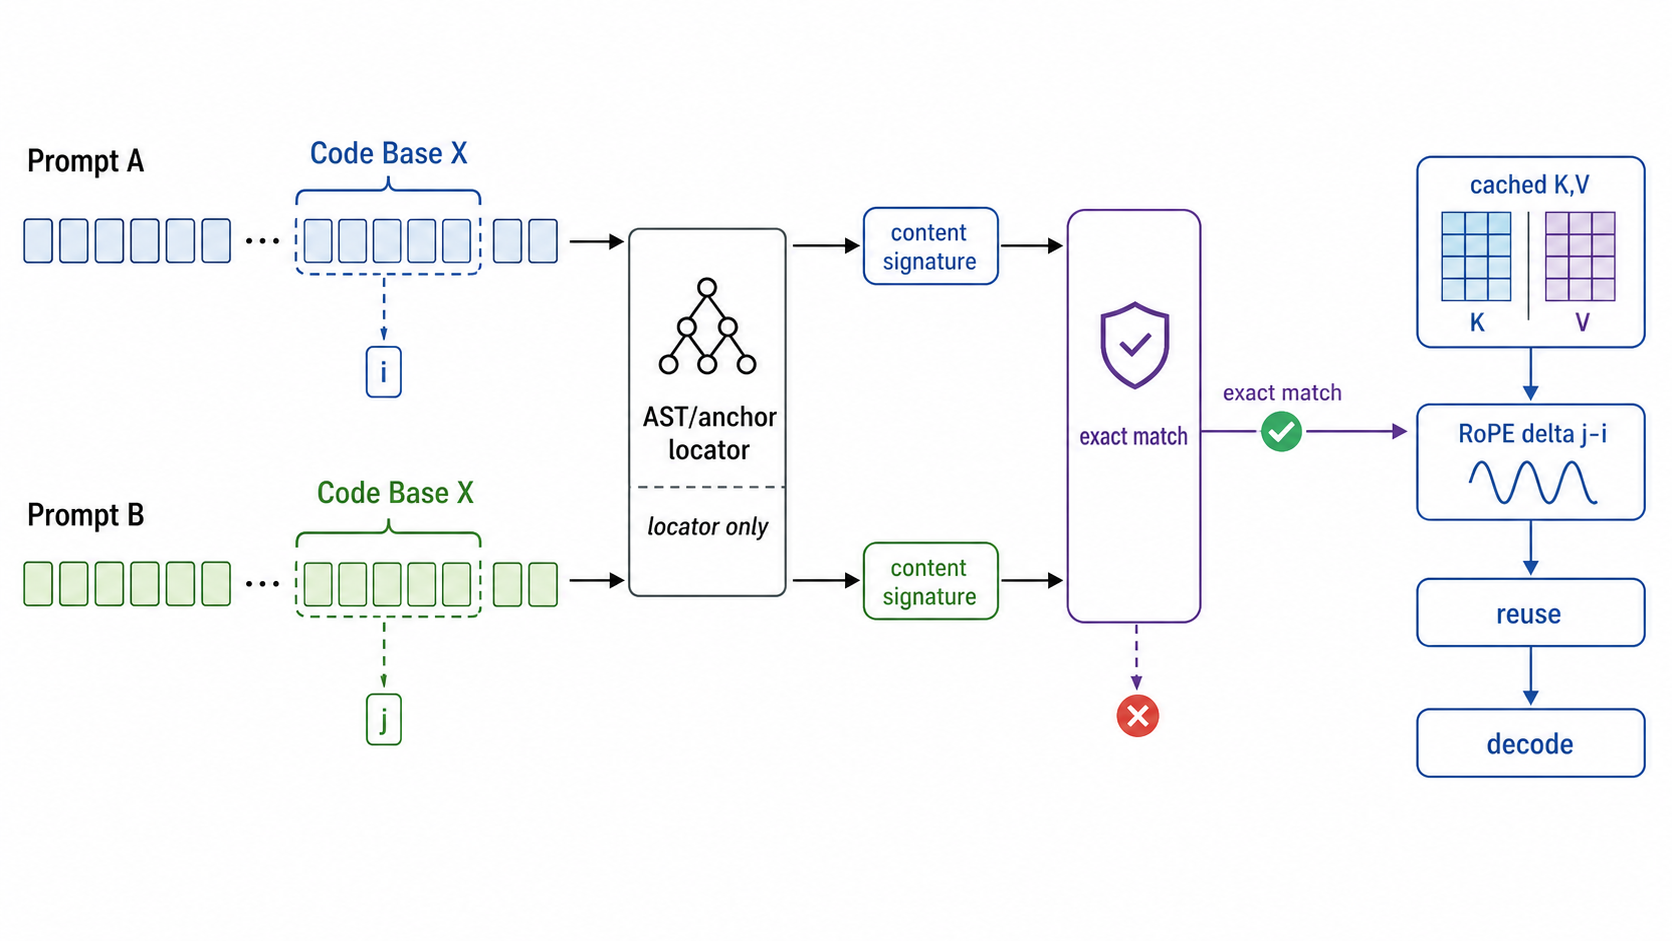
\includegraphics[width=\columnwidth]{figures/fig_kvcomm_mechanism.png}
  \caption{Exact-content segment reuse. AST/anchor information locates candidate spans only; reuse requires exact code content and then applies RoPE delta alignment for the target prompt position.}
  \Description{Two prompts contain the same code base at different positions; AST anchors locate spans, content signatures gate reuse, and RoPE delta transforms cached K,V.}
  \label{fig:kvcomm}
\end{figure}

\subsection{Safety Invariant}

\system enforces a single safety invariant:
\[
\mathrm{reuse\_allowed} \Rightarrow
\mathrm{match\_reason}=\mathrm{exact\_code\_content\_signature}.
\]
This invariant rules out AST-only, path-only, function-name-only, and span-overlap-only reuse.
It also makes the system robust to malicious or accidental near matches.
The invariant is checked at the last possible moment, after tokenization and after candidate lookup.
This placement prevents the system from depending on agreement between the MAS controller and the serving runtime.
If a template claims that a future agent will reuse a code object but the actual prompt contains a modified version, the signature comparison fails and the request is served through normal prefill.
If a cache entry is absent or evicted, the invariant is vacuously preserved because no reuse occurs.
